%% ============================================
%% 115年度教育部教學實踐研究計畫
%% 參、教學設計與規劃
%% ============================================

\subsection{教學設計與規劃}

\paragraph{教學理念與設計原則}

本研究之教學設計以「AI鷹架漸退模式」為核心,融合三大理論框架:自我調節學習理論(Self-Regulated Learning,SRL)\cite{zimmerman2002becoming}、認知學徒制(Cognitive Apprenticeship)\cite{collins1989cognitive}與問題導向學習(Problem-Based Learning,PBL)\cite{savery2006overview}。設計原則如下:

\textbf{原則一:結構化AI支持}

相關研究顯示\cite{kazemitabaar2024codeaid},採用「不直接提供完整程式碼」的AI鷹架設計,透過概念解釋、虛擬碼生成、錯誤標註等方式提供分層支持,能有效促進學生學習並避免過度依賴。本課程據此設計AI工具為學習引導者而非答案提供者。

\textbf{原則二:漸進式鷹架撤除}

依據認知學徒制相關文獻\cite{collins1989cognitive}的「示範-指導-鷹架-漸退」模式,本課程將AI支持程度從高(引導期)逐步降至低(自主期)。另有研究指出\cite{wood1976role},鷹架的核心精神在於初期提供支持、隨能力增長逐步撤除,促進學習者內化知識與技能。

\textbf{原則三:問題導向情境學習}

多項研究顯示\cite{hmelo2004problem},PBL能有效促進深度學習、問題解決能力與自主學習動機;在臺灣脈絡下的教學實踐亦證實\cite{lin2021teaching},結合PBL與翻轉教室於程式設計課程能顯著提升成效與動機。本課程每週以真實程式設計問題為導向,增進學習動機與知識遷移。

\textbf{原則四:自我調節學習培養}

有研究將SRL定義為學習者主動設定目標、監控歷程、調整策略的循環過程\cite{zimmerman2002becoming};亦有研究指出在科技輔助學習環境中,SRL能力是學習成功的關鍵預測因子\cite{azevedo2019using}。本課程透過學習反思報告、AI使用紀錄回顧等活動,引導學生發展後設認知能力。

\paragraph{課程架構概述}

本課程為期\textbf{18週},每週\textbf{3小時},共計\textbf{54小時}。課程設計分為兩大部分:

\textbf{第一部分:Python基礎知識建構(第1-9週)}

課程架構參考哈佛大學CS50P(CS50's Introduction to Programming with Python)的設計\cite{cs50p2024},涵蓋Python程式設計核心知識:函式與變數、條件判斷、迴圈、例外處理、套件、檔案處理等基礎概念。此部分著重建立學生的程式設計基礎能力。

\textbf{第二部分:問題解決與專題應用(第10-18週)}

運用前9週所學的Python基礎知識,透過真實問題情境與專題實作,培養學生的問題解決能力、知識整合能力與自主學習能力。此部分著重將所學知識應用於實際問題,並逐步撤除AI鷹架,達成研究目標。

課程分為三個教學階段,配合AI鷹架漸退設計:

\begin{figure}[htbp]
  \centering
  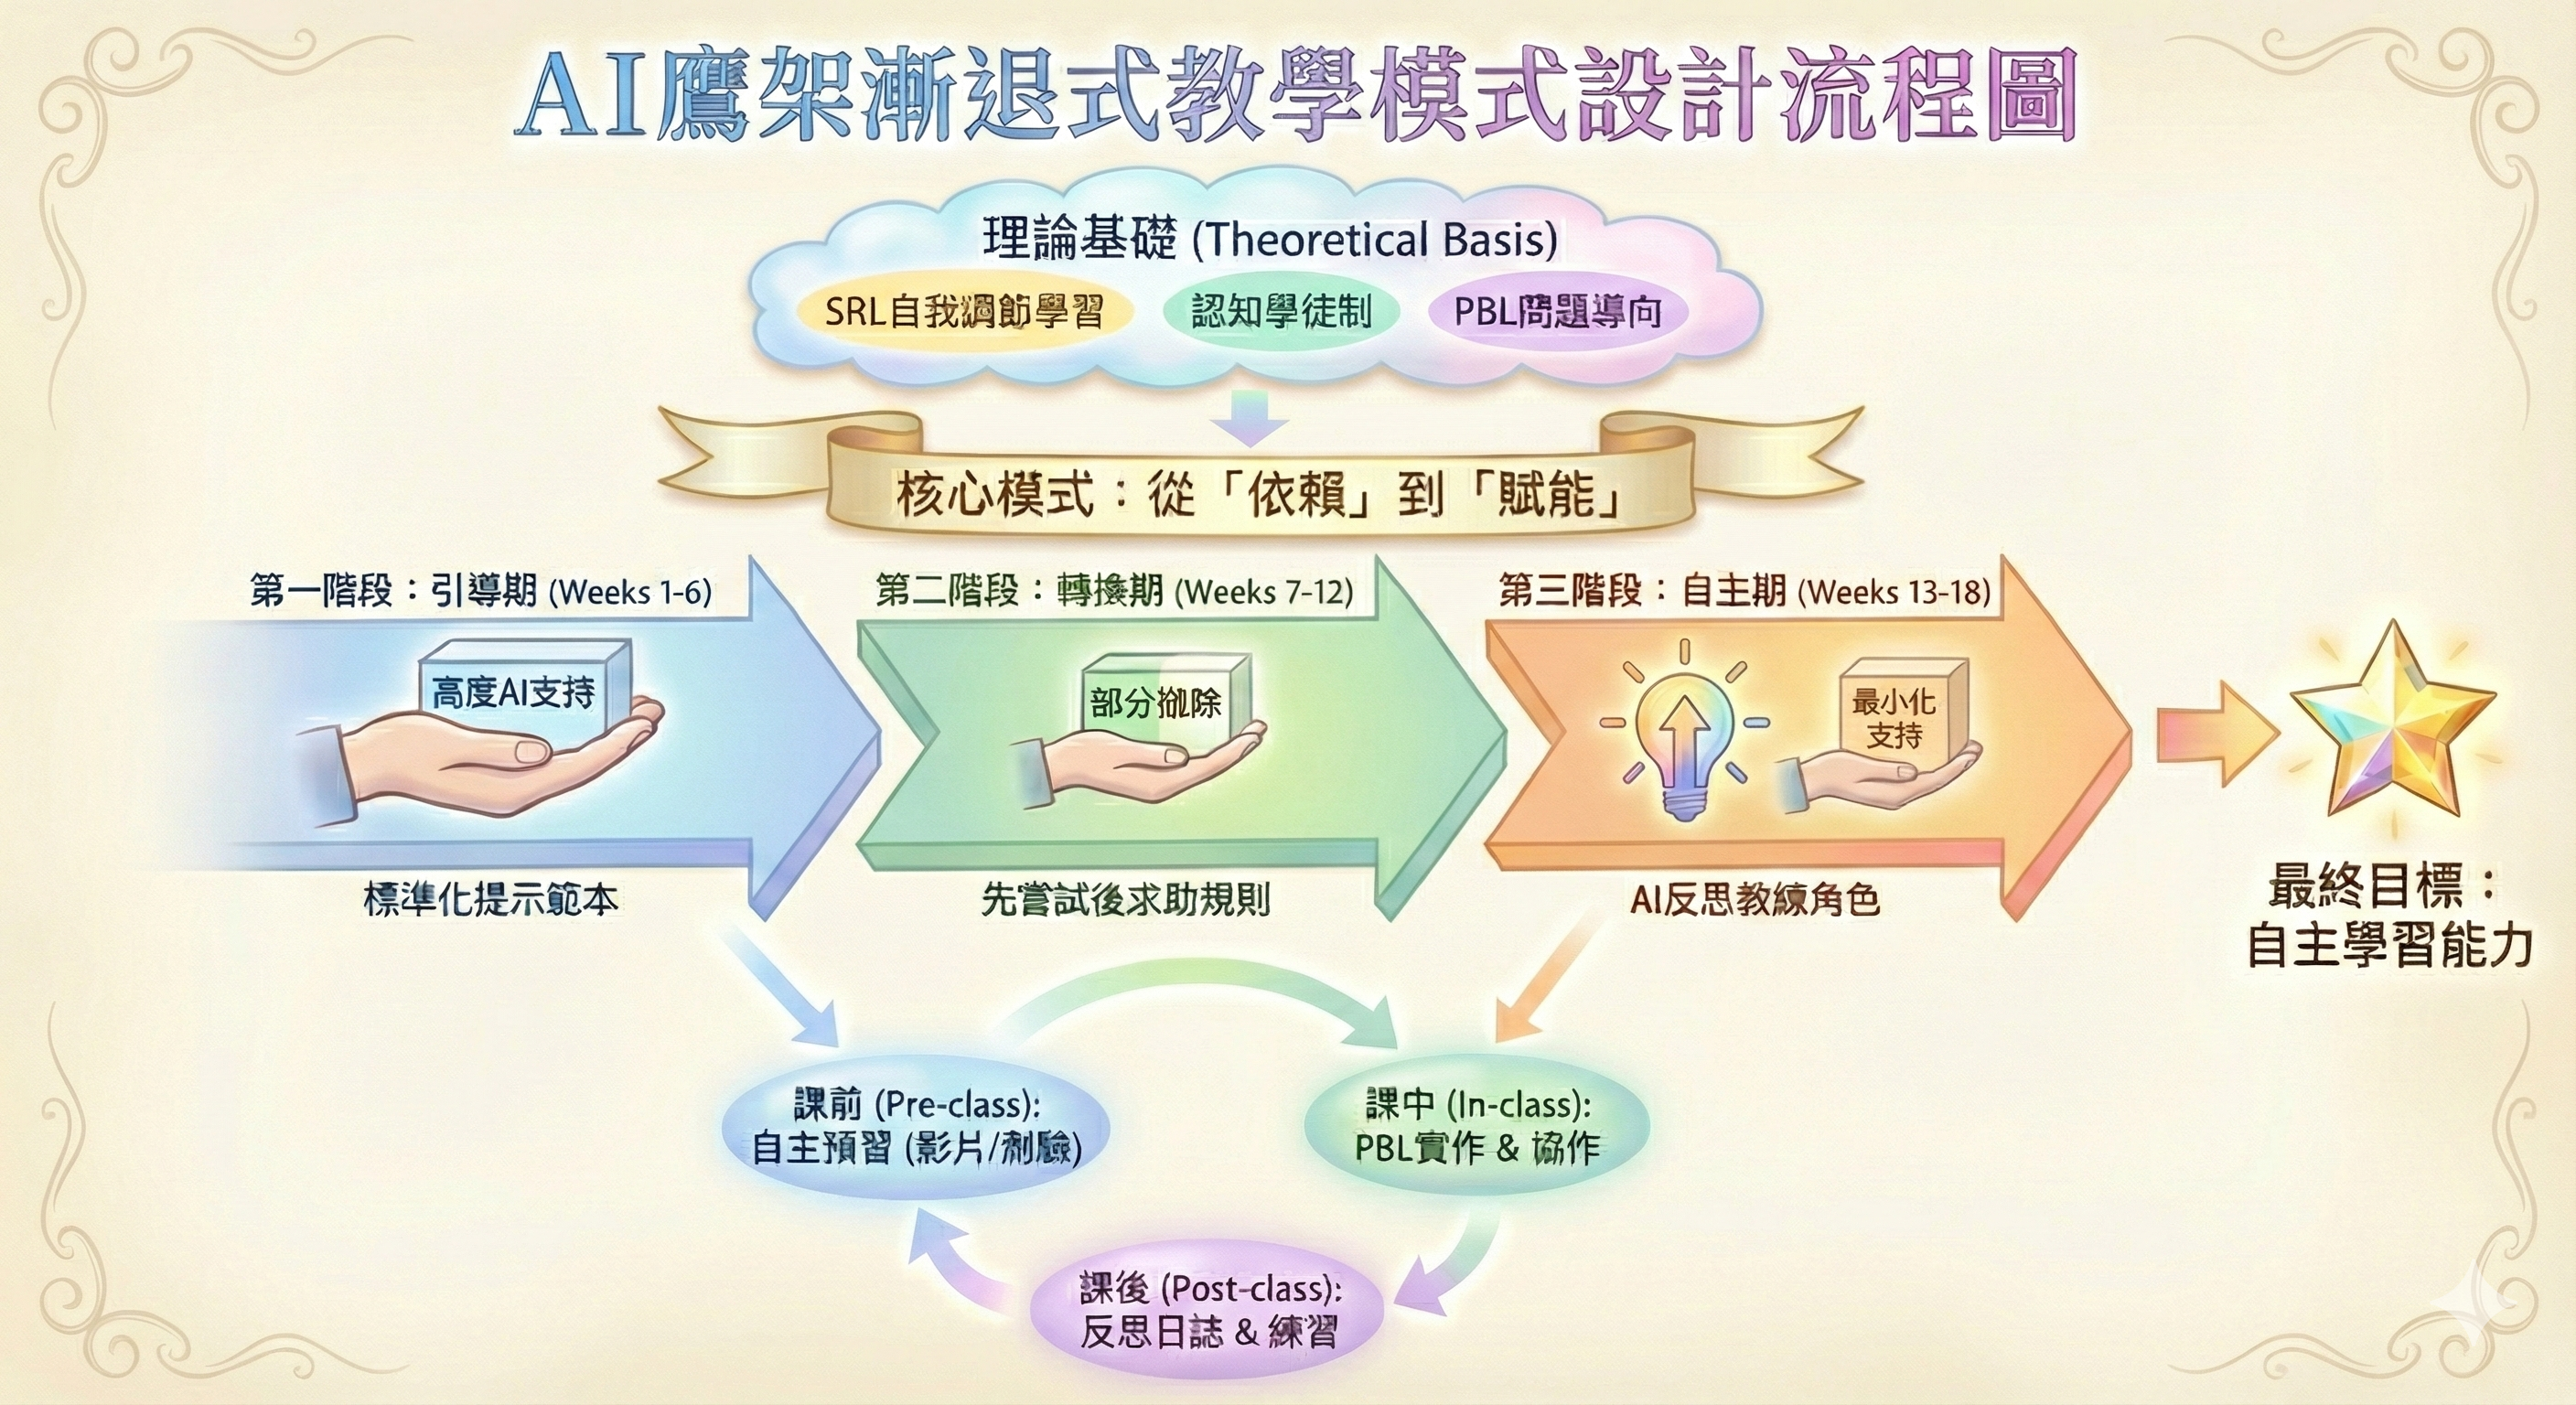
\includegraphics[width=0.9\linewidth]{teaching_flow.png}
  \caption{AI鷹架漸退教學模式}
  \label{fig:teaching_flow}
\end{figure}

\begin{table}[h]
\centering
\caption{三階段課程架構與研究目標對應}
\renewcommand{\arraystretch}{1.25}
\begin{tabular}{|c|c|m{4.5cm}|m{4.5cm}|}
\hline
\textbf{階段} & \textbf{週次} & \textbf{課程重點} & \textbf{對應研究目標} \\
\hline
引導期 & 1-6週 & Python基礎知識(CS50P核心內容) & 建立基礎能力、學習AI使用策略 \\
\hline
轉換期 & 7-12週 & 進階知識與問題解決應用 & 減少AI依賴、培養獨立思考 \\
\hline
自主期 & 13-18週 & 專題實作與知識整合 & 建立自主學習能力、完成專題 \\
\hline
\end{tabular}
\end{table}

\paragraph{18週課程設計}

\paragraph{第一階段:引導期(1-6週)}

\textbf{教學目標}:
\begin{itemize}[leftmargin=2em]
\item 建立Python程式設計基礎概念與語法
\item 學習有效使用AI工具的策略與提示工程技巧
\item 培養程式設計的基本問題解決思維
\end{itemize}

\textbf{AI鷹架設計}:高度結構化支持
\begin{itemize}[leftmargin=2em]
\item 提供標準化提示範本(prompt templates),引導學生正確提問方式
\item AI回應包含三層次:概念解說→虛擬碼引導→思考提問
\item AI不直接輸出完整程式碼,要求學生根據提示自行實作
\item 錯誤診斷模式:AI指出錯誤類型與可能原因,不直接提供修正版本
\end{itemize}

\textbf{週次規劃}:

\begin{table}[h]
\centering
\caption{引導期週次規劃}
\renewcommand{\arraystretch}{1.25}
\begin{tabular}{|c|m{3cm}|m{4cm}|m{5cm}|}
\hline
\textbf{週次} & \textbf{主題} & \textbf{CS50P對應內容} & \textbf{課堂活動} \\
\hline
1 & 課程介紹與環境設定 & Week 0: Functions(1/2) & 認識Python、安裝環境、第一支程式 \\
\hline
2 & 變數與資料型別 & Week 0: Variables(2/2) & 變數宣告、資料型別、輸入輸出、前測施測 \\
\hline
3 & 條件判斷 & Week 1: Conditionals & if-elif-else、布林運算、邏輯判斷 \\
\hline
4 & 迴圈結構 & Week 2: Loops & while迴圈、for迴圈、range函式 \\
\hline
5 & 函式設計 & Week 0: Functions(進階) & 函式定義、參數傳遞、回傳值 \\
\hline
6 & 資料結構基礎 & Week 2: Lists & 串列、字典、基本操作、第一次量表施測 \\
\hline
\end{tabular}
\end{table}

\paragraph{第二階段:轉換期(7-12週)}

\textbf{教學目標}:
\begin{itemize}[leftmargin=2em]
\item 學習進階Python概念與技術
\item 培養獨立思考與問題解決能力
\item 減少對AI工具的依賴程度
\end{itemize}

\textbf{AI鷹架設計}:部分撤除支持
\begin{itemize}[leftmargin=2em]
\item 移除標準化提示範本,鼓勵學生自行設計提示詞
\item 建立「先嘗試後求助」規則:學生需先獨立嘗試15分鐘再使用AI
\item AI回應轉為「問題診斷」模式,提供方向性建議而非具體解法
\item 引入同儕協作機制:參考社會性共享調節概念之相關研究\cite{jarvela2015enhancing}
\end{itemize}

\textbf{週次規劃}:

\begin{table}[h]
\centering
\caption{轉換期週次規劃}
\renewcommand{\arraystretch}{1.25}
\begin{tabular}{|c|m{3cm}|m{4cm}|m{5cm}|}
\hline
\textbf{週次} & \textbf{主題} & \textbf{CS50P對應內容} & \textbf{課堂活動} \\
\hline
7 & 例外處理 & Week 3: Exceptions & try-except、錯誤類型、防禦性程式設計 \\
\hline
8 & 套件應用 & Week 4: Libraries & 第三方套件、pip安裝、API串接 \\
\hline
9 & 檔案處理 & Week 6: File I/O & 檔案讀寫、CSV處理、資料存取 \\
\hline
10 & 問題解決實作(一) & 綜合應用 & 整合Week 0-6知識解決實際問題 \\
\hline
11 & 問題解決實作(二) & 綜合應用 & 小組協作解決複雜問題、期中專題規劃 \\
\hline
12 & 期中專題發表 & 綜合應用 & 專題報告、同儕互評、第二次量表施測 \\
\hline
\end{tabular}
\end{table}

\paragraph{第三階段:自主期(13-18週)}

\textbf{教學目標}:
\begin{itemize}[leftmargin=2em]
\item 整合所學知識完成期末專題
\item 建立自主學習能力與後設認知
\item 培養程式設計的持續學習態度
\end{itemize}

\textbf{AI鷹架設計}:最小化支持
\begin{itemize}[leftmargin=2em]
\item AI角色轉變為「反思教練」(reflection coach)
\item 不主動提供程式建議,僅回應學生明確且具體的提問
\item 重點功能:引導學生回顧學習歷程、檢視學習策略、自我評估
\end{itemize}

\textbf{週次規劃}:

\begin{table}[h]
\centering
\caption{自主期週次規劃}
\renewcommand{\arraystretch}{1.25}
\begin{tabular}{|c|m{3cm}|m{4cm}|m{5cm}|}
\hline
\textbf{週次} & \textbf{主題} & \textbf{學習重點} & \textbf{課堂活動} \\
\hline
13 & 進階主題(一) & Week 7: Regular Expressions & 正規表示式、文字處理應用 \\
\hline
14 & 進階主題(二) & Week 8: OOP基礎概念 & 類別與物件基本概念(簡化版) \\
\hline
15 & 期末專題規劃 & 專題設計 & 專題選題、需求分析、架構設計 \\
\hline
16 & 期末專題實作(一) & 專題開發 & 核心功能開發、問題解決 \\
\hline
17 & 期末專題實作(二) & 專題完善 & 功能完善、測試除錯、後測施測 \\
\hline
18 & 期末專題發表 & 成果展示 & 專題報告、同儕互評、第三次量表施測 \\
\hline
\end{tabular}
\end{table}

\paragraph{每週課堂活動設計}

每週3小時課程採用「課前-課中-課後」三段式設計:

\textbf{課前活動}(自主學習約30分鐘):
\begin{itemize}[leftmargin=2em]
\item 觀看教師錄製的概念講解影片(10-15分鐘)
\item 完成線上預習測驗
\item 記錄預習疑問點
\end{itemize}

\textbf{課中活動}(面對面教學3小時):
\begin{itemize}[leftmargin=2em]
\item 概念澄清與重點講解(30分鐘):針對預習問題進行解答
\item 範例示範與練習(60分鐘):教師示範、學生跟做練習
\item PBL任務實作(60分鐘):小組協作解決本週程式設計任務
\item 成果分享與反思(30分鐘):小組報告、教師回饋、學習反思
\end{itemize}

\textbf{課後活動}(自主學習約60分鐘):
\begin{itemize}[leftmargin=2em]
\item 完成延伸練習題
\item 撰寫AI使用紀錄與學習反思(每4週繳交一次正式報告)
\end{itemize}

\paragraph{PBL任務設計}

本課程PBL任務設計強調三大核心能力:「資料處理」、「資料視覺化」與「真實問題解決」。基礎練習題(如變數運算、迴圈練習、函式撰寫等)已融入每週課堂練習中,PBL任務則聚焦於具有挑戰性的應用問題。任務設計結合「Vibe Coding」理念——鼓勵學生以自然語言描述需求,透過與AI協作逐步實現程式功能,培養人機協作的程式開發能力。

\paragraph{核心技術能力培養}

本課程PBL任務涵蓋以下技術能力:

\begin{itemize}[leftmargin=2em]
\item \textbf{資料處理}:CSV/JSON檔案讀取、資料清理、資料轉換、資料篩選與彙整
\item \textbf{資料視覺化}:使用Matplotlib、Pandas繪製統計圖表(長條圖、折線圖、圓餅圖、散佈圖)
\item \textbf{API串接}:呼叫政府開放資料API、處理JSON回應、錯誤處理
\item \textbf{問題解決}:需求分析、演算法設計、程式實作、測試除錯
\end{itemize}

\paragraph{臺灣開放資料應用}

本課程大量採用「政府資料開放平臺」(data.gov.tw)之公開資料集,讓學生處理真實、在地化的資料,提升學習動機與實用性。使用之資料集包括:

\begin{itemize}[leftmargin=2em]
\item 中央氣象署開放資料:天氣預報、地震資訊、雨量觀測
\item 交通部開放資料:YouBike即時資訊、公車動態、臺鐵時刻
\item 環境部開放資料:空氣品質AQI、紫外線指數
\item 衛生福利部開放資料:醫療院所、食品營養成分
\item 內政部開放資料:人口統計、行政區域資訊
\item 花蓮縣政府開放資料:在地觀光景點、活動資訊
\end{itemize}

\paragraph{Vibe Coding教學策略}

「Vibe Coding」強調以直覺、自然的方式與AI協作開發程式,本課程將此理念融入PBL任務:

\begin{itemize}[leftmargin=2em]
\item \textbf{引導期}:教師示範如何用自然語言描述需求,AI協助產生程式框架,學生理解並修改
\item \textbf{轉換期}:學生自行撰寫需求描述,批判性評估AI建議,選擇性採納並改進
\item \textbf{自主期}:學生主導開發流程,AI僅作為諮詢對象,培養獨立解決問題能力
\end{itemize}

\paragraph{PBL任務一覽}

\begin{table}[htbp]
\centering
\caption{PBL任務設計一覽表}
\renewcommand{\arraystretch}{1.3}
\small
\begin{tabular}{|c|p{2.8cm}|p{5cm}|p{3.8cm}|}
\hline
\textbf{週次} & \textbf{PBL任務名稱} & \textbf{任務說明} & \textbf{技術重點} \\
\hline
\multicolumn{4}{|c|}{\textbf{引導期:結構化AI協作任務}} \\
\hline
6 & 花蓮空氣品質監測儀表板 & 讀取環境部AQI資料,根據空氣品質等級提供健康建議,並繪製AQI趨勢圖 & 資料處理、條件判斷、Matplotlib折線圖 \\
\hline
\multicolumn{4}{|c|}{\textbf{轉換期:半自主問題解決任務}} \\
\hline
9 & 花蓮YouBike使用分析系統 & 串接YouBike API,分析各站點使用率,繪製站點分布圖與使用統計 & API串接、資料清理、長條圖與圓餅圖 \\
\hline
10 & 臺灣人口結構視覺化分析 & 讀取內政部人口統計CSV,分析各縣市人口結構、年齡分布,產生多種統計圖表 & CSV處理、Pandas資料分析、多圖表繪製 \\
\hline
11--12 & 期中專題:在地生活資料應用 & 整合至少兩種開放資料,進行資料處理與視覺化分析,解決在地生活問題 & 多元資料整合、資料視覺化、小組協作 \\
\hline
\multicolumn{4}{|c|}{\textbf{自主期:獨立專題開發任務}} \\
\hline
13 & 新聞/社群文字資料探勘 & 使用正規表示式擷取網路文字資料,進行詞頻統計與視覺化呈現 & 正規表示式、文字處理、詞頻統計圖 \\
\hline
14 & 地震資料分析與視覺化系統 & 串接氣象署地震開放資料,分析地震分布規律,繪製地震規模統計圖 & API串接、OOP概念、散佈圖與統計分析 \\
\hline
15--18 & 期末專題:自選主題 & 自選臺灣開放資料主題,完成資料蒐集、處理、分析與視覺化呈現 & 完整資料分析流程、全方位知識整合 \\
\hline
\end{tabular}
\end{table}

\paragraph{期末專題建議方向}

學生可從以下方向選擇期末專題主題,皆須包含資料處理與視覺化分析:

\begin{enumerate}
\item \textbf{環境分析類}:空氣品質趨勢分析、氣溫變化視覺化、紫外線指數統計
\item \textbf{交通分析類}:YouBike使用熱點分析、公車路線效率評估、交通流量視覺化
\item \textbf{人口社會類}:縣市人口趨勢分析、年齡結構變化圖、人口密度地圖
\item \textbf{健康飲食類}:食品營養成分比較、醫療資源分布分析、健康指標統計
\item \textbf{觀光旅遊類}:花蓮景點分析、觀光人次趨勢、旅遊資源視覺化儀表板
\end{enumerate}
